\batchmode
\documentclass{beamer}
\usepackage[utf8]{inputenc}
\usepackage[T1]{fontenc}
\usepackage[ngerman]{babel}
\usepackage{amsmath}

\usetheme[deutsch]{KIT}
\author{Jan Haag (jan.haag@student.kit.edu)}
\title{Programmieren Tutorium 11 -- Interfaces und Generics}
\institute{Institut f\"{u}r Zeritfizierbare und Vertrauensw\"{u}rdige Informatiksysteme (ZVI)}
\TitleImage[scale=0.225]{frontpic.jpg}

\begin{document}
\begin{frame}
\maketitle
\end{frame}

\begin{frame}
\frametitle{Inhalt}
\tableofcontents
\end{frame}

\section{Interfaces}
\begin{frame}[fragile]
\frametitle{Interfaces}
\begin{itemize}
\item Enthalten Konstanten und Methoden
\item Alle Methoden Abstrakt
\item Erben nur von Interfaces
\pause
\item Mehrfachvererbung sicher
\end{itemize}
\end{frame}

\begin{frame}[fragile]
\frametitle{Interfaces}
\begin{verbatim}
public interface Interface extends Cloneable {
    public static final int CONSTANT = 0;
    public boolean foo();
}

public class Bar implements Interface {
    @Override
    public boolean foo() {
        return false;
    }
}
\end{verbatim}
\end{frame}

\section{Generics}
\begin{frame}[fragile]
\frametitle{Generics}
\begin{itemize}
\item Verhindert Codeduplikate
\item Typsicher (meistens)
\item Pr\"{u}fung der Typen durch Compiler (oder auch nicht!)
\end{itemize}
\pause
\verb|http://goo.gl/ZumuL|, Section 4.4
\end{frame}

\subsection{Generics -- Typische Fehler}
\begin{frame}[fragile]
\frametitle{Vergessene Typerweiterung}
\begin{verbatim}
LinkedList is = new LinkedList<Integer>();
\end{verbatim}
\end{frame}

\begin{frame}[fragile]
\frametitle{Unchecked-Warnung abgeschaltet}
\begin{verbatim}
@SuppressWarnings("unchecked")
public LinkedList foo() {
    LinkedList<Integer> is = new LinkedList();
    // Do something
    return is;
}

@SuppressWarnings("unchecked")
public void bar() {
    LinkedList<Float> = foo();
}
\end{verbatim}
\end{frame}

\section{Aufgabe}
\begin{frame}[fragile]
\frametitle{Aufgabe}
\textbf{Functional Programming in Java!}\\\vspace{1\baselineskip}
\pause
Implementieren Sie ein Interface \verb|FancyList|, das sich an das
Interface \verb|java.util.List| h\"{a}lt und ausserdem die Funktionen
\verb|foldr|, \verb|foldl|, \verb|map| und \verb|filter| definiert.
Implementieren Sie eine FancyList unter Verwendung von Vererbung.
Schreiben Sie dazu Interfaces \verb|Function1| und \verb|Function2|,
die eine Funktion mit einem bzw. zwei Parametern darstellen.
\end{frame}

\begin{frame}[fragile, shrink]
\frametitle{Definitionen}
\begin{verbatim}
foldr :: (a -> b -> b) -> b -> [a] -> b
foldr f x [] = x
foldr f x (y:ys) = f y (foldr f x ys)

foldl :: (b -> a -> b) -> b -> [a] -> b
foldl f x [] = x
foldl f x (y:ys) = f (foldl f x ys) y

map :: (a -> b) -> [a] -> [b]
map f xs = foldr transform xs []
    where transform elem buf = (f elem) : buf

filter :: (a -> Bool) -> [a] -> [a]
filter p xs = foldr transform xs []
    where transform elem buf | p elem = elem : buf
                             | otherwise = buf
\end{verbatim}
\end{frame}

\begin{frame}[fragile]
\frametitle{Ende}
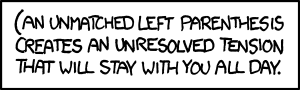
\includegraphics[scale=1.0]{(.png}\\\vspace{1\baselineskip}
<<\verb|Brains aside, I wonder how many poorly-written|\\
\verb|xkcd.com-parsing scripts will break on this title|\\
\verb|(or \;;";\''{<<;[' this mouseover text.";|>>
\end{frame}
\end{document}
